\section{Dynamic-MSV-Bench and Methodology}
\label{sec:benchmark}

We propose the \textbf{Dynamic-MSV-Bench}, which categorizes multi-shot prompts into two rigorous evaluation scenarios to systematically expose the "Double-Kill" dilemma prevalent in current generative models.

\begin{figure*}[ht]
    \centering
    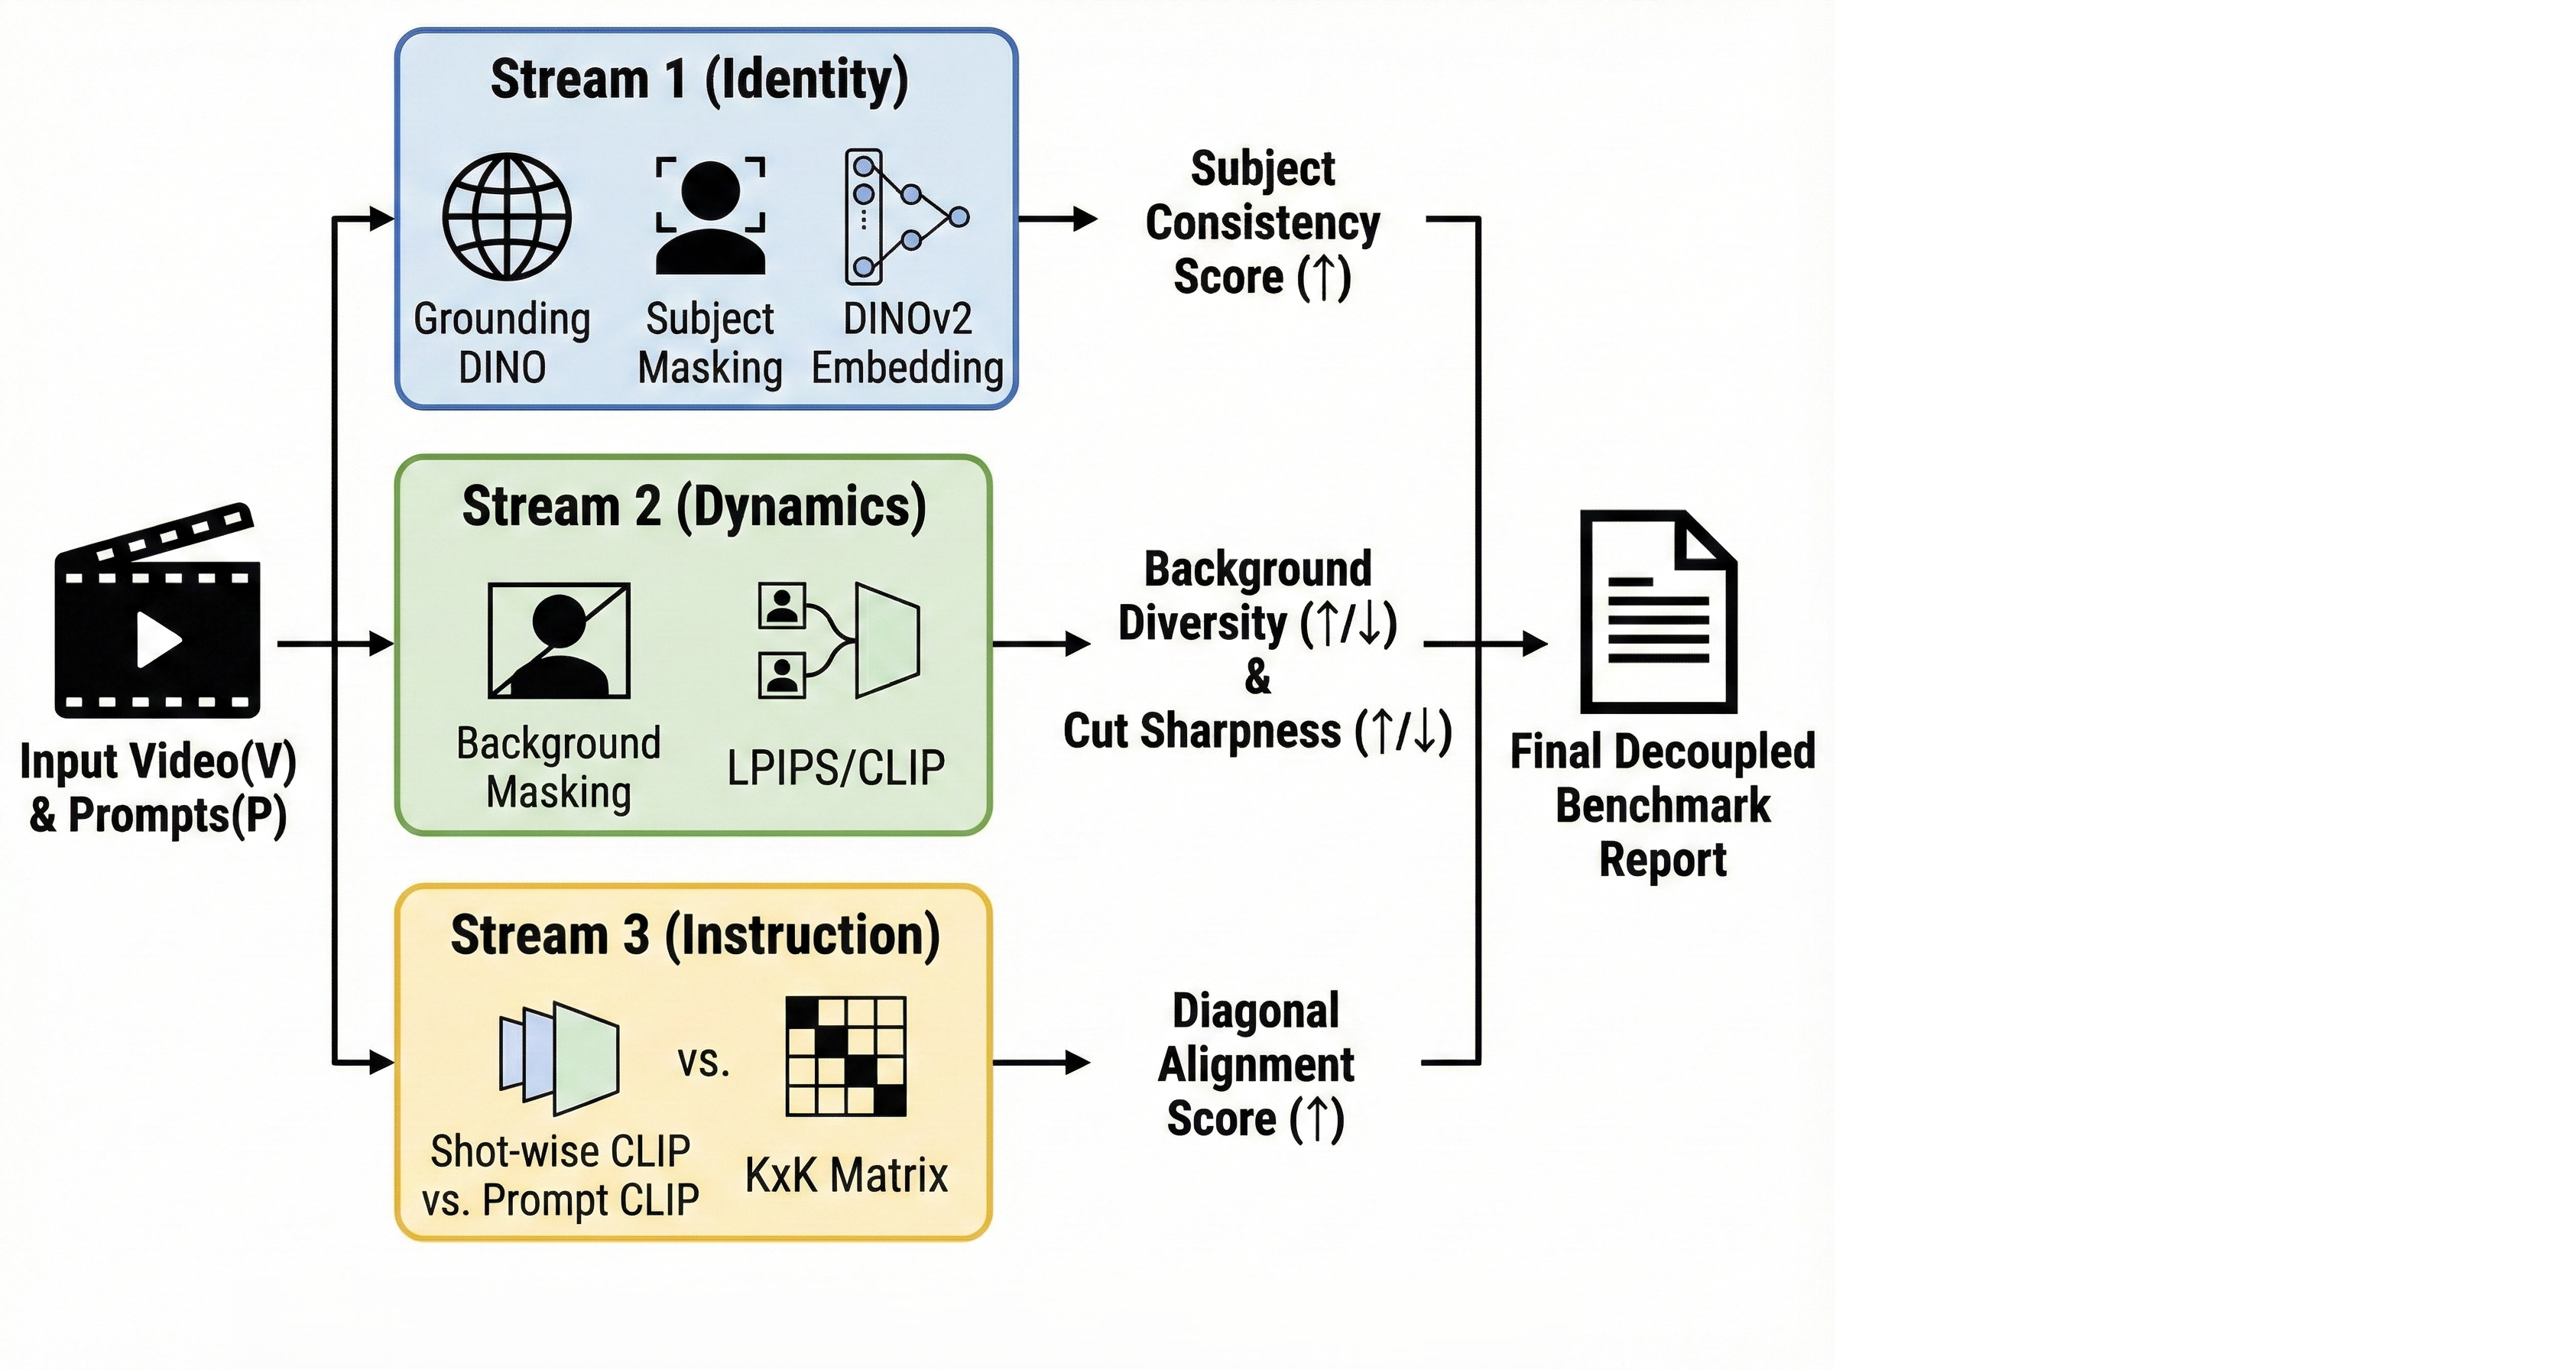
\includegraphics[width=\textwidth]{figures/images/fig2.png}
    \caption{Overview of our Decoupled 4D Evaluation Framework. Unlike holistic metrics like FVD, we process the input video through three independent streams to measure Subject Identity, Background Dynamics/Continuity, and Instruction Following (Diagonal Alignment) separately. This decoupling allows for scenario-aware evaluation (Track S vs. Track M).}
    \label{fig:framework}
\end{figure*}

\begin{figure*}[ht]
    \centering
    \includegraphics[width=\textwidth]{figures/images/fig_AB.jpg}
    \caption{Conceptual comparison of our two evaluation tracks. (Left) \textbf{Track S: Semantic Leap} tests narrative diversity, requiring radical environment changes while preserving the subject. (Right) \textbf{Track M: Motion Continuity} evaluates spatial integrity, where the background must remain consistent while the camera executes specific motions.}
    \label{fig:sets_comparison}
\end{figure*}

\subsection{Track S: Semantic Leap (Narrative Diversity)}
Track S evaluates the model's ability to maintain a consistent subject while drastically shifting the semantic environment. The \textbf{Golden Rule for Track S} is defined as HIGH Background Diversity ($\uparrow$), HIGH Cut Sharpness ($\uparrow$), HIGH Subject Consistency ($\uparrow$), and HIGH Diagonal Semantic Alignment (DSA, $\uparrow$).

\begin{itemize}
    \item \textbf{Background Diversity ($\uparrow$):} Since the narrative requires a leap between disparate locations, the model must exhibit high variance in its environmental rendering. A low score here directly exposes the \textit{Static Trap}.
    \item \textbf{Cut Sharpness ($\uparrow$):} Jumps should be depicted as distinct cinematic cuts, preventing unnatural "morphing" artifacts.
    \item \textbf{Subject Consistency ($\uparrow$):} The identity of the main protagonist must remain strictly preserved across the leap.
    \item \textbf{Diagonal Semantic Alignment ($\uparrow$):} The model must explicitly follow the unique semantic instructions of each shot, guaranteeing the shift is driven by the prompt rather than context bleeding.
\end{itemize}

\subsection{Track M: Motion Continuity (Spatial Integrity)}
Track M tests physical instructions while keeping the background spatially stable. The \textbf{Golden Rule for Track M} is defined as LOW Background Diversity ($\downarrow$), LOW Cut Sharpness ($\downarrow$), HIGH Subject Consistency ($\uparrow$), and HIGH Diagonal Semantic Alignment (DSA, $\uparrow$).

\begin{itemize}
    \item \textbf{Background Diversity ($\downarrow$):} The background must remain pixel-consistent while the camera moves. High diversity indicates \textit{Background Hallucination}.
    \item \textbf{Cut Sharpness ($\downarrow$):} Transitions between camera actions (e.g., pan to zoom) should be spatially continuous, rewarding a single, cohesive 3D space.
    \item \textbf{Subject Consistency ($\uparrow$):} The protagonist must be preserved throughout the changes in perspective.
    \item \textbf{Diagonal Semantic Alignment ($\uparrow$):} Even with a static background, the model must accurately differentiate between fine-grained camera control instructions.
\end{itemize}

\subsection{Taxonomy of Failure Modes}
Our benchmark uniquely identifies systemic failures by cross-referencing metrics across tracks. Table~\ref{tab:failure_taxonomy} summarizes the key signals used to profile current T2MSV models.

\begin{table}[ht]
\centering
\caption{Taxonomy of T2MSV Failure Modes. We identify the "Static Trap" and "Identity Amnesia" by analyzing the divergence between Diversity and Consistency across Track S and Track M.}
\label{tab:failure_taxonomy}
\resizebox{\linewidth}{!}{
\begin{tabular}{l|ccc}
\toprule
\textbf{Failure Mode} & \textbf{Track S (Leap)} & \textbf{Track M (Continuity)} & \textbf{Key Metric Signal} \\
\midrule
\textbf{Static Trap} & Div. $\downarrow$, Cons. $\uparrow$ & Div. $\downarrow$, Cons. $\uparrow$ & $DSA \approx 0$ (Both) \\
\textbf{Identity Amnesia} & Div. $\uparrow$, Cons. $\downarrow$ & Div. $\uparrow$, Cons. $\downarrow$ & Cons. $\downarrow$ in Track S \\
\midrule
\textbf{Ideal Target} & Div. $\uparrow$, Cons. $\uparrow$ & Div. $\downarrow$, Cons. $\uparrow$ & High $DSA$ (Both) \\
\bottomrule
\end{tabular}}
\end{table}

\subsection{The 4D Decoupled Metrics}
Our framework utilizes four specialized indices to quantitatively decompose performance.

\subsubsection{Subject Consistency ($\mathcal{C}_{subj}$)}
We utilize a masked DINOv2 similarity to measure identity preservation across $K$ shots:
$$\mathcal{C}_{subj} = \frac{2}{K(K-1)} \sum_{i < j} \cos(\Phi_{DINO}(s_i \odot m_i), \Phi_{DINO}(s_j \odot m_j))$$

\subsubsection{Background Diversity ($\mathcal{D}_{bg}$)}
To identify the \textit{Static Trap}, we measure the variance of the background environment embeddings ($\overline{m}_i$):
$$\mathcal{D}_{bg} = 1 - \left( \frac{1}{K^{2}}\sum_{i,j} \cos(\Phi(s_{i}\odot\overline{m}_{i}), \Phi(s_{j}\odot\overline{m}_{j})) \right)$$

\subsubsection{Cut-Transition Sharpness ($\mathcal{S}_{cut}$)}
We quantify the distinctness of shot boundaries using LPIPS distance peaks:
$$\mathcal{S}_{cut} = \text{LPIPS}(f_{t_{cut}-1}, f_{t_{cut}+1})$$

\subsubsection{Diagonal Semantic Alignment (DSA)}
Our core novelty measures the independent adherence to shot-level instructions. We apply a column-wise softmax with logit scaling $\tau$ to the shot-prompt similarity matrix $M$:
$$P_{i,j} = \frac{\exp(\tau \cdot M_{i,j})}{\sum_{k=1}^{K} \exp(\tau \cdot M_{k,j})}, \quad DSA = \max \left( 0, \frac{\frac{1}{K}\sum_{i=1}^{K} P_{i,i} - \frac{1}{K}}{1 - \frac{1}{K}} \right)$$
As visualized in Figure~\ref{fig:dsa_heatmaps}, a static video yields a DSA of exactly 0.0.

\begin{figure*}[ht]
    \centering
    \includegraphics[width=\textwidth]{figures/dsa_heatmaps_phd.pdf}
    \caption{Diagonal Semantic Alignment (DSA) Heatmaps. (A) Models in the \textbf{Static Trap} show a uniform probability distribution. (B) Models with \textbf{Context Bleeding} show noisy diagonal alignment. (C) An \textbf{Ideal Decoupled Model} exhibits sharp, precise shot execution.}
    \label{fig:dsa_heatmaps}
\end{figure*}
